\section{Threat Model}
\label{sec:threat}
% tikz is loaded in the preamble of the main file. Packages must not sit in the body.
% Source of truth, threat-models.agents.md and formal_verif.threat-model.agents.md.
% Limitations belong to the Discussion, not here.
A confidentiality claim about a compiler is empty until three questions have been answered.
Who is watching, what is that observer after, and at which stage of the toolchain the leak appears.
The first answer follows the usual practice of ranking observers by
how directly they reach secret state rather than by how powerful they
are assumed to be: side-channel taxonomies place attackers by
proximity~\cite{spreitzer2018classification}, and constant-time
leakage models nest so that a proof against a stronger observation
carries over to weaker ones~\cite{molnar2005pcmodel,almeida2016ctverif}.
We arrange eight such observers in rings so that every verdict in this
paper can be pinned to one.
The second question is where deep learning parts company with cryptography, because the assets of a model deployment are exposed on a schedule no cipher is ever exposed on, and it is that schedule, not the width of the channel, which decides what counts as a leak worth fixing.
The third question allows an observed channel to be charged to the source or to the compiler, which is the distinction our four-valued verdicts rest on.
Two of our findings are caused unambiguously by the compiler, neither of them is observed while a program runs, and so persistence is named here as a leak class of its own, which may be found only after execution ends.
\subsection{Observers}
\label{sec:threat:rings}
An observer is fixed by two things, the channel it reads, functional or timing or microarchitectural or power, and its position with respect to the secret.
For position we use eight rings, ordered so that every observer that infers sits outside every observer that reads.
Table~\ref{tab:rings} lists them and Fig.~\ref{fig:onion} draws the same ordering as nested reach. An observer placed on an outer ring holds strictly less than one placed inside it. The dashed circle marks where inference stops being necessary rather than where it stops being possible, since an observer inward of it already reads process memory.
\begin{figure}[t]
\centering
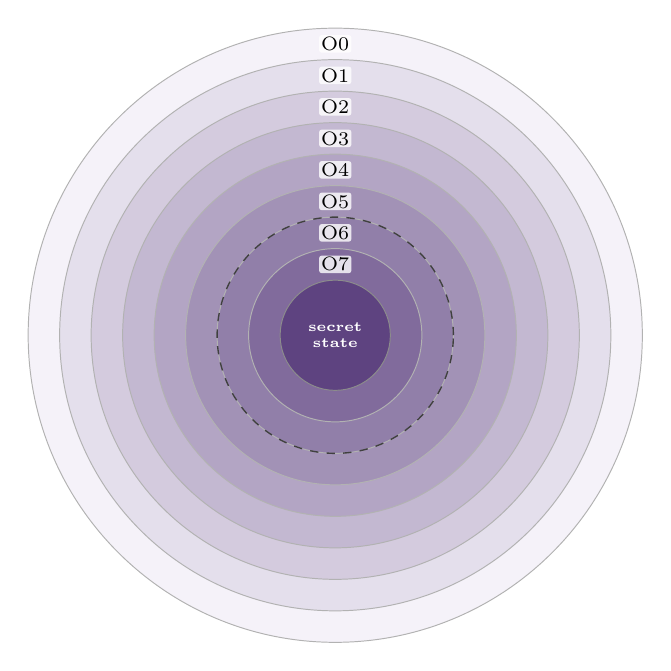
\begin{tikzpicture}[font=\scriptsize,line width=0.35pt]
  \definecolor{ringout}{HTML}{F5F2F9}
  \definecolor{ringin}{HTML}{5E4380}
  \foreach \i in {0,...,7} {
    \pgfmathsetmacro{\r}{3.90-\i*0.40}
    \pgfmathsetmacro{\mix}{11*\i}
    \fill[ringin!\mix!ringout,draw=black!30] (0,0) circle (\r);
  }
  \fill[ringin,draw=black!45] (0,0) circle (0.70);
  \foreach \i/\lab in {0/O0,1/O1,2/O2,3/O3,4/O4,5/O5,6/O6,7/O7} {
    \pgfmathsetmacro{\y}{3.90-\i*0.40-0.20}
    \node[inner sep=0.8pt,fill=white,fill opacity=0.80,text opacity=1,
          rounded corners=1pt] at (0,\y) {\lab};
  }
  \node[white,align=center,font=\tiny\bfseries] at (0,0) {secret\\state};
  \draw[dashed,black!75,line width=0.5pt] (0,0) circle (1.50);
\end{tikzpicture}
\caption{An observer model}
\label{fig:onion}
\end{figure}
\begin{table}[t]
\caption{Observer rings, ordered by directness of reach.}
\label{tab:rings}
\centering
\small
\begin{tabular}{@{}l@{\hspace{1em}}p{0.78\columnwidth}@{}}
\hline
ring & what the observer holds \\
\hline
O0 & outputs, errors, response length \\
O1 & latency measured end to end, repeated query statistics \\
O2 & branches, address classes, latency classes \\
O3 & cache sets and lines, pages, predictors, contention \\
O4 & power, EM, acoustic, thermal, frequency \\
O5 & the powers of a host minus whatever an enclave declares unreachable \\
O6 & process memory, registers, logs, files, core dumps \\
O7 & buses, internal memories, chip probes \\
\hline
\end{tabular}
\end{table}

A property proved at O2 carries outward to O1 and to O0.
A property that fails at O3 fails at O4 and at O5 as well, since the outer observer holds everything the inner one holds and more.
Inward of O6 the question dissolves rather than staying open, because an observer that already reads process memory has nothing left to infer.
Every verdict below is stated against a ring, and the two halves of the paper meet at O2, where the measurements bound the channel from below and the proofs discharge it from above.
A ring says how much an observer can see.
It does not say what a single operation gives away, and that finer vocabulary is what the leakage model of our checker supplies, sorting observations into the control, address, latency and resource obligations of \S\ref{sec:verify}.
The two are one axis read at two granularities.
The ring is the unit in which a verdict is stated and an attack is priced, the obligation kind is the unit in which a verdict is discharged and a channel is named, and a control obligation or an address obligation is nothing other than an O2 observation refined into the operand that produces it.
\subsection{Which asset, and therefore whether repetition helps}
\label{sec:threat:asset}
O2 is precisely the ring that classical constant-time discipline addresses, since the discipline demands that the sequence of branches and the sequence of memory addresses be independent of the secret, and it is that discipline our proofs discharge.
What the discipline assumes without saying so is that the secret is ephemeral.
A session key is used a bounded number of times and then discarded, so a channel yielding a small fraction of a bit per execution recovers nothing before the secret has gone.
A model deployment breaks the assumption, and it breaks it in opposite directions for the two assets that matter.
Weights are frozen, and every forward pass re-exposes the same secret.
A weak and noisy channel together with ordinary API access is therefore sufficient, because the attacker averages until the channel is clean.
Time works for him rather than against him, and a leak a cryptographer would dismiss as unexploitable is decisive here.
Recovery of architecture and of weights from cache~\cite{yan2020cachetelepathy}, from architectural observation~\cite{hu2020deepsniffer} and from electromagnetic observation~\cite{batina2019csinn} all run on this budget.
Inputs are the mirror image.
A token id is seen once, repetition buys nothing, and so the channel has to resolve the secret inside a single execution, which happens exactly when the leak is address shaped and the secret is small.
An embedding row gather at a secret token id is the clean case.
A single cache line observation narrows a vocabulary of thousands of entries substantially, in one query, with no averaging at all.
The two assets therefore do not merely differ in value, they make different leaks matter.
Variable latency arithmetic on a weight is a slow grind that repetition eventually wins.
A gather on a token id is immediate.
A third asset sits between the two and behaves like neither.
The architecture itself, together with tensor shapes, extents and sparsity or pruning patterns, is static and coarse, and it leaks through control structure rather than through values, which makes it invisible to any instrument that follows value flow and plainly visible in the address channel of a sparsity aware lowering.
It is also the asset the compiler reaches first, and the case studies below are where that shows: a secret extent used as a loop bound stays control-flow distinguishable at every pipeline and optimization level we tested, and sparsification moves a secret coordinate into a store address while leaving every aggregate count identical.
\subsection{Persistence, the attacker who arrives after the run}
\label{sec:threat:persistence}
Rings O0 to O5 all describe an observer of a running program, and each
of them needs co-residency or query access. An observer of the
persistent output of the compiler needs neither. The artifact exists
before the program has ever been run, it survives every run, and
reading it costs one call to \texttt{open}. Constant folding under
weight freezing writes a scale derived from $\max|w|$ into the generated
code as a literal, so whoever reads the artifact recovers that scale
exactly, without running the kernel and without timing anything. This
is not an accident of one optimization but the general shape of
quantized deployment: narrow numeric formats cannot represent a
tensor's dynamic range, so every quantized tensor ships a scale computed
from its largest magnitude, per tensor for int8 and
FP8~\cite{fp8formats}, per block of sixteen elements for
NVFP4~\cite{nvfp4} and thirty-two for MX~\cite{ocpmx}. Each scale is a function of the largest
magnitude in its scope, the maximum itself for per-tensor formats, an
FP8 value derived from it for NVFP4 and its exponent for MX, stored apart from the weight data and carried
through the pipeline as metadata. The folded literal we measure in
\S\ref{sec:production} is one instance of a statistic that every such
deployment writes into its artifact by design. Ahead-of-time
compilation goes further and bakes raw weight bytes into a shared
object that sits under a directory chain traversable by others and
outlives the compiling process.
 
Shapes leak by a parallel route. A compiler that specializes a tensor
dimension to a constant fixes that size into the generated code, so a
size derived from a protected extent becomes a secret written into the
artifact: the dynshape kernel of \S\ref{sec:evaluation:structure}, one level up. A
compiler that specializes must also re-check its assumption on every
call, a runtime comparison on the architecture
asset~\cite{pytorch2}. The two routes are not arbitrary. A compiler
reasons about a program on tensors that carry shapes but no data, so
anything it can derive from shape alone can be fixed into the artifact,
while anything that depends on the values reaches it only through a
deliberate exception. The artifact holds a program's shapes by default
and its weights only when the compiler is told to treat them as
constants.
 
None of these leaks is functional, since nothing was returned, nor
timing, since nothing was timed. No shared hardware state is involved,
so none is microarchitectural, and nothing was measured through power.
The closest fit in the ring vocabulary is O6, which does list files,
but O6 is moot by the argument above, and an attacker who can open a
file under a different UID holds no process memory whatsoever. That
attacker is strictly weaker than O6 and unlike anything in O0 to O5.
The standard grid conflates two entirely different observers, and our
clearest compiler-introduced results fall into the gap between them. We
therefore add persistence as a leak class, defined by the single
property that separates it from the other four: the attacker arrives
later, and reads rather than watches. It has two subcases. Build-time
residue is the artifact. Runtime residue is memory, swap, core dumps,
spilled registers, a reused connection pool, or GPU scratch left behind
for the next tenant.
 
Runtime residue is also a compiler problem, and for a structural
reason. A program that clears a secret before releasing its buffer
writes to memory that nothing reads again; to the abstract machine the
language defines, that store is dead, and removing it is a correct
optimization. Dead-store elimination does exactly this to scrubbing
code, a case D'Silva, Payer and Song place at the centre of the gap
between compiler correctness and security~\cite{dsilva2015gap}.
Yodaiken makes the general point from the side of systems programming:
the language standard, not the programmer's intent, decides what a
compiler may remove, and what systems code relies on the standard often
does not guarantee~\cite{yodaiken2021iso}. MLIR is no different, since
a deallocation promises nothing about the contents it releases. This is
why correctness of a lowering, the property the verifiers of
\S\ref{sec:verify} inherit, cannot rule out a persistence leak.
 
Naming the class rather than filing it under the nearest ring is the
same discipline this paper applies to what its methods cannot state: a
gap that is reported is a different object from a gap that has been
quietly counted as secure.
\subsection{Where this bites}
\label{sec:threat:deployments}
Four deployments fix different combinations of asset, observer and leak class.
The first is confidential inference inside a TEE.
The weights are the asset, the observer is O5 and close to an oracle, since controlled channel attacks resolve at the granularity of a 4 KB page~\cite{xu2015controlled} and single stepping resolves per instruction~\cite{vanbulck2017sgxstep}, and weight confidentiality is the guarantee the deployment advertises, so a secret dependent gather is a direct break and not a hypothetical one.
The second is multi-tenant serving, where both assets are present with opposite economics, where the observers are O3 and a persistence reader, and where one asymmetry decides everything.
The platform compiles, so the platform picks the optimization flags, the cache directory and the umask, while the tenant owns the weights and picks none of the three.
The third is on device and edge deployment.
Here the adversary owns the hardware, holds O3, O4, O6 and O7 and holds the artifact as well, and the honest aim is to raise cost rather than to close the channel.
The fourth is compiling for obliviousness.
The job of the compiler is then to emit data oblivious code, a leak is not an accident of optimization but a correctness bug inside a security mechanism, and this is why pass by pass verdicts are directly actionable.
When one pass closes an address channel while another opens a control channel, only the whole pipeline is safe, and whoever runs the first pass alone is not.
